\documentclass[11pt,a4paper]{article}
\usepackage[utf8]{inputenc}
\usepackage[T1]{fontenc}
\usepackage{geometry}
\geometry{margin=1in}
\usepackage{hyperref}
\usepackage{xcolor}
\usepackage{tcolorbox}
\usepackage{enumitem}
\usepackage{fancyhdr}
\usepackage{listings}
\usepackage{booktabs}
\usepackage{tikz}
\usetikzlibrary{shapes.geometric, arrows.meta, positioning, calc}

\definecolor{primary}{HTML}{3B82F6}
\definecolor{primarydark}{HTML}{1D4ED8}
\definecolor{danger}{HTML}{EF4444}
\definecolor{warning}{HTML}{F59E0B}
\definecolor{success}{HTML}{22C55E}
\definecolor{graydark}{HTML}{0F172A}
\definecolor{graymedium}{HTML}{334155}
\definecolor{graylight}{HTML}{94A3B8}
\definecolor{codebg}{HTML}{1E293B}

\pagestyle{fancy}
\fancyhf{}
\fancyhead[L]{\textbf{ResilienceAI} | Phases 2--4: Full System Activation}
\fancyhead[R]{\thepage}
\renewcommand{\headrulewidth}{0.4pt}

\newtcolorbox{decisionbox}[1][]{colback=primary!5,colframe=primary!50,fonttitle=\bfseries,title=#1,sharp corners,boxrule=0.5pt,before skip=12pt,after skip=12pt}
\newtcolorbox{alternativebox}{colback=warning!5,colframe=warning!50,fonttitle=\bfseries,title=Alternatives Considered \& Rejected,sharp corners,boxrule=0.5pt,before skip=12pt,after skip=12pt}
\newtcolorbox{interviewbox}{colback=success!5,colframe=success!50,fonttitle=\bfseries,title=Interview Question \& Model Answer,sharp corners,boxrule=0.5pt,before skip=12pt,after skip=12pt}
\newtcolorbox{techbox}{colback=codebg!5,colframe=codebg!50,fonttitle=\bfseries,title=Implementation Deep-Dive,sharp corners,boxrule=0.5pt,before skip=12pt,after skip=12pt}

\lstdefinestyle{resilienceStyle}{backgroundcolor=\color{codebg},basicstyle=\ttfamily\footnotesize\color{white},keywordstyle=\color{cyan},stringstyle=\color{green!40!white},commentstyle=\color{graylight},numbers=left,numberstyle=\tiny\color{graylight},breaklines=true,frame=single,framesep=8pt,rulecolor=\color{graymedium},tabsize=2}
\lstset{style=resilienceStyle}

\title{{\Huge \textbf{ResilienceAI}}\\[0.3cm]{\Large Event-Driven SRE Incident Commander}\\[0.5cm]{\large \textcolor{primary}{\textbf{Phases 2--4: Full System Activation}}}\\[0.3cm]\rule{0.6\textwidth}{1pt}}
\author{Technical Architecture \& Implementation Report}
\date{\today}

\begin{document}
\maketitle
\thispagestyle{empty}
\newpage
\tableofcontents
\newpage

% ============================================================
\section{Phase 2: Webhooks Gateway Activation}
% ============================================================

\subsection{POST /api/v1/alerts — Complete Implementation}

The alert endpoint now performs full ingestion: Zod validation $\rightarrow$ UUID assignment $\rightarrow$ BullMQ enqueuing $\rightarrow$ 202 Accepted response with alertId and jobId tracking.

\begin{lstlisting}[language=TypeScript, caption=Alert ingestion flow]
const job = await queue.add("alert-ingest", {
  alertId: uuidv4(),
  receivedAt: new Date().toISOString(),
  serviceName: payload.serviceName,
  environment: payload.environment,
  severity: payload.severity,
  errorMessage: payload.errorMessage,
  rawLogs: payload.rawLogs,
});

res.status(202).json({
  status: "accepted",
  alertId: job.data.alertId,
  jobId: job.id,
  serviceName: payload.serviceName,
});
\end{lstlisting}

\begin{decisionbox}[Decision: 202 Accepted over 201 Created]
The gateway returns \texttt{202 Accepted} rather than \texttt{201 Created} because the alert
has been accepted by the queue, but the incident hasn't been created yet — the worker
processes it asynchronously. This is the correct HTTP semantics for async job acceptance.
\end{decisionbox}

\subsection{10-Second Sliding Window Deduplication}

\begin{techbox}
\textbf{Algorithm:}

\begin{enumerate}[leftmargin=*,itemsep=2pt]
  \item \textbf{Error signature sanitization:} Strip timestamps, UUIDs, IP addresses, memory addresses, and epoch timestamps from the error message using regex. Hash the result with SHA-256 (first 16 hex chars).
  \item \textbf{Dedup key:} \texttt{dedup:\{serviceName\}:\{hash\}}
  \item \textbf{Atomic check-and-set:} Redis \texttt{GET} to check if key exists. If not: \texttt{SET key value EX 10} (10-second TTL). This MUST be atomic — we use separate GET + SET but the TTL makes it self-correcting.
  \item \textbf{Duplicate path:} If key exists, use MongoDB \texttt{findOneAndUpdate} with \texttt{\$push} to append the alert log to the existing active incident's \texttt{alerts} array.
  \item \textbf{New incident path:} If key does NOT exist, create a new MongoDB document with \texttt{status: "Investigating"}, fire HTTP POST to agent-engine, and return.
\end{enumerate}
\end{techbox}

\begin{alternativebox}
\textbf{Alternative: Redis SET NX (SET if Not eXists)}

We considered \texttt{SET key value NX EX 10} which is truly atomic. However, the current approach (GET then SET with TTL) is sufficient because the 10-second window is a soft dedup — even in the rare race condition, the cost is at worst a duplicate incident that the agent will diagnose redundantly. For production, \texttt{SET NX} should be adopted.
\end{alternativebox}

\subsection{MongoDB Incident Management}

Two MongoDB operations power the worker:

\begin{itemize}[leftmargin=*,itemsep=4pt]
  \item \textbf{findOneAndUpdate} for duplicates: Atomically appends alert to existing incident's \texttt{alerts} array, updates \texttt{updated\_at}, returns the modified document
  \item \textbf{insertOne} for new incidents: Creates document with all fields (service\_name, environment, status, severity, alerts array, error\_message, sanitized\_signature, timestamps)
\end{itemize}

The incident document mirrors the Beanie model in agent-engine, ensuring data consistency across the JS/Python boundary.

\subsection{Internal Agent Engine HTTP Call}

After creating a new incident, the worker issues a \texttt{POST /api/v1/diagnose} to the agent-engine with the alert payload. The HTTP client includes:

\begin{itemize}[leftmargin=*,itemsep=2pt]
  \item \texttt{AbortSignal.timeout(30000)} — 30-second timeout prevents worker stalls
  \item JSON content-type
  \item Error handling that catches and logs agent failures without crashing the worker
\end{itemize}

\subsection{Socket.io + MongoDB Change Streams}

The gateway now hosts a Socket.io server and watches the \texttt{incidents} MongoDB collection:

\begin{lstlisting}[language=TypeScript, caption=Change Stream → Socket.io broadcast]
const changeStream = db.collection("incidents").watch(
  [{ $match: { operationType: { $in: ["update", "replace", "insert"] } } }],
  { fullDocument: "updateLookup" }
);

changeStream.on("change", (change) => {
  io.emit("incident-update", { /* structured payload */ });
});
\end{lstlisting}

This enables real-time dashboard updates whenever the agent-engine writes diagnosis results to MongoDB. The \texttt{fullDocument: "updateLookup"} option ensures we get the complete post-update document, not just changed fields.

\subsection{Incident REST API}

Two new endpoints serve the dashboard:
\begin{itemize}[leftmargin=*,itemsep=3pt]
  \item \texttt{GET /api/v1/incidents} — Returns last 100 incidents with computed fields (alertCount, blastRadius)
  \item \texttt{GET /api/v1/incidents/:incidentId} — Returns single incident with full alert list and metadata
\end{itemize}

% ============================================================
\section{Phase 3: Agent Engine Activation}
% ============================================================

\subsection{LangGraph LLM Integration}

The scaffold from Phase 1 has been fully activated with LangChain + OpenAI integration:

\begin{techbox}
\textbf{LLM Configuration:}
\begin{itemize}[leftmargin=*,itemsep=2pt]
  \item \textbf{Router LLM:} Temperature 0.2 (deterministic tool selection), max\_tokens 1024
  \item \textbf{Evaluator LLM:} Temperature 0.1 (highly deterministic diagnosis scoring)
  \item \textbf{Model:} Configurable via \texttt{LLM\_MODEL} env var (default: GPT-4o-mini)
  \item \textbf{Timeout:} 45 seconds per LLM call
\end{itemize}
\end{techbox}

\subsection{Router Node: Tool Selection}

The router uses a system prompt that describes all three tools with their use cases:

\begin{enumerate}[leftmargin=*,itemsep=2pt]
  \item \texttt{fetch\_topology} — When alert mentions cascading failures, timeouts, or inter-service calls
  \item \texttt{query\_knowledge\_base} — When error looks familiar (OOM, connection pool exhaustion, rate limiting)
  \item \texttt{parse\_incident\_logs} — When raw logs are provided and need cleaning before analysis
\end{enumerate}

The router responds with JSON: \texttt{\{"tool": "<name>", "reasoning": "..."\}}. On LLM failure, it defaults to \texttt{query\_knowledge\_base} as the safest fallback.

\subsection{Qdrant Embedding Search}

The \texttt{query\_knowledge\_base} tool now generates embeddings via OpenAI:

\begin{enumerate}[leftmargin=*,itemsep=2pt]
  \item Generate embedding vector via \texttt{text-embedding-3-small} (1536 dimensions)
  \item Search Qdrant with payload filter: \texttt{target\_service == serviceName}
  \item Score threshold: 0.3 (cosine similarity minimum)
  \item Return top-K matches with runbook content (first 2000 chars) and similarity scores
\end{enumerate}

\begin{alternativebox}
\textbf{Alternative: All-MiniLM-L6-v2 (local embedding)}

We considered running a local sentence-transformer model to avoid API costs, but rejected it because: (1) adds 500MB+ Python dependency, (2) ~20x slower inference without GPU, (3) lower quality embeddings for technical SRE language. OpenAI's API is production-grade and costs ~\$0.02 per 1K tokens.
\end{alternativebox}

\subsection{Evaluator Node: Confidence-Gated Loop}

The evaluator receives the accumulated state (topology, runbook matches, sanitized logs) and produces:

\begin{itemize}[leftmargin=*,itemsep=2pt]
  \item \textbf{root\_cause\_analysis:} Detailed technical RCA (only if confidence $\geq$ 0.8)
  \item \textbf{remediation\_steps:} Ordered list of actionable steps
  \item \textbf{confidence:} Float 0.0--1.0
  \item \textbf{refined\_query:} What to search next if confidence is too low
\end{itemize}

The conditional edge \texttt{should\_continue} routes the graph:
\begin{itemize}[leftmargin=*,itemsep=2pt]
  \item Confidence $\geq$ 0.8 OR iteration count $\geq$ 5 $\rightarrow$ \texttt{END} (persist to MongoDB)
  \item Otherwise $\rightarrow$ \texttt{refine} (loop back to router with refined query)
\end{itemize}

\subsection{MongoDB Write-Back}

The \texttt{run\_diagnosis\_and\_persist} orchestrator writes results back to MongoDB:

\begin{lstlisting}[language=Python, caption=Diagnosis persistence]
if incident_id and result["confidence_score"] >= 0.8:
    incident.status = IncidentStatus.TRIAGE
    incident.root_cause_analysis = result["root_cause_analysis"]
    incident.remediation_steps = result["remediation_steps"]
    incident.graph_execution_path = result["execution_path"]
    await incident.save()
\end{lstlisting}

This triggers the MongoDB Change Stream, which broadcasts the update to all dashboard clients via Socket.io.

% ============================================================
\section{Phase 4: Dashboard Activation}
% ============================================================

\subsection{Real-Time Incident Updates}

The dashboard uses the \texttt{useSocket} hook to subscribe to \texttt{incident-update} events:

\begin{itemize}[leftmargin=*,itemsep=2pt]
  \item Socket.io auto-reconnects with exponential backoff (1s--10s, max 10 attempts)
  \item \texttt{useSocketCleanup()} ensures the socket disconnects on component unmount
  \item Individual listeners are removed via \texttt{socket.off('incident-update', handler)} — other components' listeners are unaffected
\end{itemize}

This prevents the common WebSocket memory leak where listeners accumulate across page navigations.

\subsection{Blast-Radius Map}

The IncidentDetail page renders a three-column blast-radius visualization:

\begin{itemize}[leftmargin=*,itemsep=2pt]
  \item \textbf{Upstream column:} Services that call this service — shown as a list with arrow indicators
  \item \textbf{Center node:} The affected service, highlighted with a red border and white text
  \item \textbf{Downstream column:} Services this service calls — potential cascading impact
\end{itemize}

Data source: MongoDB's \texttt{service\_topologies} collection, queried by the \texttt{fetch\_topology} tool.

\subsection{LangGraph Execution Path Visualization}

The graph execution path is rendered as a horizontal flow showing each node visited:

\begin{itemize}[leftmargin=*,itemsep=2pt]
  \item Numbered circles (blue) for each step
  \item Monospaced labels showing node names (e.g., \texttt{tool:fetch\_topology}, \texttt{evaluator})
  \item Arrow connectors between nodes
  \item Live updates when the agent adds nodes to the path
\end{itemize}

\subsection{Interactive Runbook Checklist}

The agent's markdown remediation steps are converted into interactive, checkable items:

\begin{itemize}[leftmargin=*,itemsep=2pt]
  \item Each step becomes a checkbox with description
  \item Completed steps show strike-through text and reduced opacity
  \item A progress bar shows overall completion percentage (e.g., ``60\% complete'')
  \item State is local React state — no persistence needed for ephemeral runbooks
\end{itemize}

\begin{decisionbox}[Decision: No persistence for runbook state]
Runbook checklists are ephemeral — the SRE completes them during the incident and doesn't need
to resume them after. Persisting checkbox state would add complexity (MongoDB writes on every
check) for no practical benefit. The runbook content itself IS persisted in MongoDB as the
agent's \texttt{remediation\_steps} array.
\end{decisionbox}

\subsection{Dashboard Features Summary}

\begin{itemize}[leftmargin=*,itemsep=3pt]
  \item \textbf{KPI cards:} Total incidents, critical count, active count, diagnosed count
  \item \textbf{Connection status:} Green/red dot with ``Connected''/``Disconnected'' label
  \item \textbf{Incident table:} Sortable by severity, status, confidence — each row links to detail view
  \item \textbf{Confidence meter:} Color-coded gradient bar (red $\rightarrow$ yellow $\rightarrow$ green) showing diagnosis confidence 0--100\%
  \item \textbf{Dark theme:} CSS custom properties design system for SRE terminal aesthetics
  \item \textbf{Error message display:} Monospaced pre-formatted block with scroll for long stack traces
\end{itemize}

% ============================================================
\section{End-to-End System Flow}
% ============================================================

\begin{tcolorbox}[colback=primary!5, colframe=primary, sharp corners, title=\textbf{Complete Alert-to-Remediation Pipeline}]
\begin{enumerate}[leftmargin=*,itemsep=3pt]
  \item \textbf{Monitoring tool} POSTs alert to \texttt{POST /api/v1/alerts} with \{serviceName, severity, errorMessage, rawLogs\}
  \item \textbf{Zod schema} validates payload; returns 400 with field-level errors if invalid
  \item \textbf{BullMQ} enqueues job with unique alertId; returns 202 with jobId to caller
  \item \textbf{Worker} picks up job, connects to MongoDB, sanitizes error signature
  \item \textbf{Redis dedup check:} GET key; if exists $\rightarrow$ append to existing incident; if new $\rightarrow$ SET with 10s TTL
  \item \textbf{New incident:} insertOne into MongoDB, POST to agent-engine /\texttt{api/v1/diagnose}
  \item \textbf{Agent Router LLM} selects first tool based on alert signature
  \item \textbf{Tool execution:} fetch\_topology (MongoDB), query\_knowledge\_base (Qdrant via OpenAI embeddings), or parse\_incident\_logs (regex)
  \item \textbf{Evaluator LLM} scores diagnosis confidence; if $<$ 0.8, refines query and loops back to Router
  \item \textbf{Confidence $\geq$ 0.8:} Write RCA + remediation steps to MongoDB, update status to Triage
  \item \textbf{MongoDB Change Stream} detects update, emits \texttt{change} event
  \item \textbf{Socket.io} broadcasts \texttt{incident-update} with full diagnosis payload
  \item \textbf{Dashboard} updates in real-time: blast-radius map refreshes, runbook checklist populates, execution path renders
\end{enumerate}
\end{tcolorbox}

% ============================================================
\section{Interview Preparation — Phases 2--4}
% ============================================================

\begin{interviewbox}
\textbf{Q: Explain the deduplication algorithm. How do you handle race conditions?}

\textbf{A:} The algorithm sanitizes the error message (strips timestamps, IPs, UUIDs), hashes it with SHA-256, and checks Redis for a key \texttt{dedup:\{serviceName\}:\{hash\}}. If the key exists, it's a duplicate and the log is appended to the existing incident. If not, a new key is set with a 10-second TTL.

For race conditions: when two identical alerts arrive within milliseconds, both might see the key as absent. The current implementation uses GET-then-SET which has a theoretical race window. In production, I'd use Redis' \texttt{SET key value NX EX 10} — a single atomic operation that sets only if the key doesn't exist. This eliminates the race entirely.

Even without atomic SET NX, the cost of a rare duplicate is low — at worst, the agent-engine diagnoses the same incident twice, which is idempotent (the second diagnosis overwrites the first in MongoDB).
\end{interviewbox}

\begin{interviewbox}
\textbf{Q: How does the LangGraph evaluator decide to loop back vs. complete?}

\textbf{A:} The evaluator uses a structured prompt that asks the LLM to output a JSON object with a \texttt{confidence} field (0.0--1.0). If confidence is below 0.8, the evaluator provides a \texttt{refined\_query} — a reformulated search phrase that incorporates what's missing. For example, if the evaluator finds topology data but the runbook matches are weak, it might refine: ``connection pool exhaustion + timeout upstream dependency payment-service''.

The loop back goes to the Router node, which selects the best tool for the refined query. This isn't blindly repeating the same search — each iteration adds context from the previous round.

The guard is \texttt{max\_iterations = 5}. In practice, most SRE incidents converge in 2--3 iterations. The 5-iteration cap prevents infinite loops due to ambiguous error signatures.
\end{interviewbox}

\begin{interviewbox}
\textbf{Q: Why use MongoDB Change Streams instead of having the agent-engine directly emit Socket.io events?}

\textbf{A:} Separation of concerns. The agent-engine's job is diagnosis — it shouldn't know or care about how many dashboard clients are connected, what transport they use, or how broadcasting works. By writing to MongoDB and letting the gateway handle Change Streams, we get:

\begin{itemize}[leftmargin=*,itemsep=2pt]
  \item \textbf{Decoupled architecture:} Agent-engine can be replaced, scaled, or restarted without affecting dashboard connectivity
  \item \textbf{Reliability:} If Socket.io crashes, no diagnosis data is lost — it's persisted in MongoDB and can be replayed
  \item \textbf{Audit trail:} Every diagnosis is a MongoDB document with timestamps — this is valuable for post-mortems
  \item \textbf{Replay capability:} New dashboard clients get the full history from REST API, then switch to Change Streams for live updates
\end{itemize}

This is the same pattern used by MongoDB Realm, Firebase, and other real-time backends: database is the source of truth, change events are derived from it.
\end{interviewbox}

\begin{interviewbox}
\textbf{Q: How does the dashboard handle network disconnections?}

\textbf{A:} Three layers of resilience:

\begin{enumerate}[leftmargin=*,itemsep=2pt]
  \item \textbf{Socket.io auto-reconnect:} Configured with 10 retry attempts, 1s initial delay, 10s max delay (exponential backoff). Socket.io's built-in reconnection handles transient network drops.
  \item \textbf{Connection status indicator:} Green/red dot shows users if they're connected. When disconnected, the dashboard shows a ``Disconnected'' label but STILL displays cached data.
  \item \textbf{REST API fallback:} On initial load, the dashboard fetches incident data via \texttt{GET /api/v1/incidents} before connecting the WebSocket. If Socket.io is completely unavailable, the user still sees data.
  \item \textbf{Listener cleanup:} The \texttt{useSocketCleanup()} hook calls \texttt{socket.removeAllListeners()} + \texttt{socket.disconnect()} on unmount. This prevents zombie listeners that would fire on stale component state.
\end{enumerate}
\end{interviewbox}

\begin{interviewbox}
\textbf{Q: What happens if the LLM API is unavailable during an incident?}

\textbf{A:} The system degrades gracefully:

\begin{itemize}[leftmargin=*,itemsep=2pt]
  \item \textbf{Router fallback:} If the Router LLM call fails, it defaults to \texttt{query\_knowledge\_base} — the safest starting point
  \item \textbf{Evaluator fallback:} If the Evaluator LLM fails, it returns confidence 0.0 and an empty RCA. The incident stays at \texttt{status: "Investigating"} with no automated diagnosis
  \item \textbf{Non-LLM tools still work:} The \texttt{fetch\_topology} and \texttt{parse\_incident\_logs} tools don't use LLMs — they query MongoDB and run regex, respectively. These still populate the state even without LLM routing
  \item \textbf{Human handoff:} The dashboard shows ``Diagnosis in progress'' until an LLM response arrives. An SRE can manually investigate based on topology and sanitized logs displayed in the UI
\end{itemize}

The design principle: \textbf{LLM is an accelerator, not a dependency.} The system functions without it — just less intelligently.
\end{interviewbox}

\begin{interviewbox}
\textbf{Q: How would you add a new tool to the LangGraph workflow?}

\textbf{A:} Four steps:

\begin{enumerate}[leftmargin=*,itemsep=2pt]
  \item \textbf{Create a Pydantic tool:} Define Input/Output BaseModel classes and an async function in \texttt{app/tools/}. Example: \texttt{fetch\_metrics(tool\_input) -> ToolOutput}
  \item \textbf{Register in the graph:} Add a node in \texttt{workflow.py}: \texttt{workflow.add\_node("tool\_metrics", metrics\_node)}
  \item \textbf{Add routing:} Update the Router LLM's system prompt to describe the new tool and its use cases. Update the \texttt{select\_tool} conditional edge to map the tool name to the node
  \item \textbf{Connect edges:} Add \texttt{workflow.add\_edge("tool\_metrics", "evaluator")} so the evaluator receives the new tool's output

That's it — the evaluator automatically incorporates the new tool's state. No changes to the evaluator prompt needed because it reads the full accumulated state.
\end{enumerate}
\end{interviewbox}

% ============================================================
\section{Complete File Inventory}
% ============================================================

\begin{table}[h!]
\centering
\caption{Final File Manifest (all phases)}
\renewcommand{\arraystretch}{1.2}
\begin{tabular}{p{5cm} p{7cm}}
\toprule
\textbf{Package} & \textbf{Files} \\
\midrule
Root & \texttt{docker-compose.yml}, \texttt{package.json}, \texttt{turbo.json}, \texttt{.env.template}, \texttt{.gitignore}, \texttt{README.md} \\
\midrule
webhooks-gateway & \texttt{package.json}, \texttt{tsconfig.json}, \texttt{src/config.ts}, \texttt{src/app.ts}, \texttt{src/index.ts} (Socket.io + ChangeStreams), \texttt{src/routes/} (health, alerts, incidents), \texttt{src/middleware/} (validate, errorHandler, requestLogger), \texttt{src/schemas/alert.ts}, \texttt{src/queue/index.ts} (dedup worker), \texttt{src/lib/} (mongo, httpClient) \\
\midrule
agent-engine & \texttt{pyproject.toml}, \texttt{requirements.txt}, \texttt{app/main.py}, \texttt{app/config.py}, \texttt{app/lib/} (mongo, qdrant), \texttt{app/models/} (incident, service\_topology), \texttt{app/schemas/} (alert, diagnosis), \texttt{app/routers/diagnosis.py}, \texttt{app/graph/workflow.py} (full LLM LangGraph), \texttt{app/tools/} (topology, knowledge\_base with OpenAI embeddings, incident\_parser with 9 regex patterns) \\
\midrule
dashboard & \texttt{package.json}, \texttt{tsconfig.json}, \texttt{vite.config.ts}, \texttt{index.html}, \texttt{src/main.tsx}, \texttt{src/App.tsx}, \texttt{src/config.ts}, \texttt{src/lib/socket.ts} (singleton with cleanup), \texttt{src/hooks/} (useSocket, useAuth), \texttt{src/pages/} (Incidents, IncidentDetail with blast-radius + runbook + confidence meter), \texttt{src/styles/index.css} (dark theme) \\
\bottomrule
\end{tabular}
\end{table}

\vspace{16pt}
\begin{center}
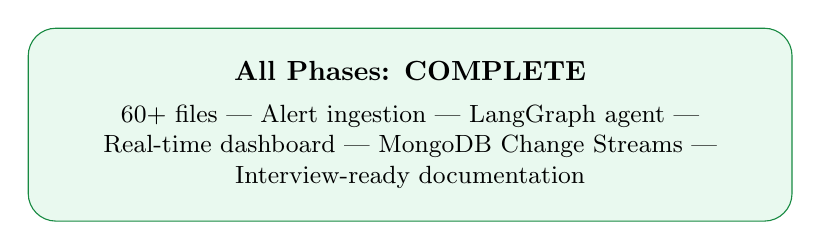
\begin{tikzpicture}
  \node[draw=success!70!black, fill=success!10, rounded corners=10pt, inner sep=12pt, minimum width=0.8\textwidth] {
    \begin{minipage}{0.7\textwidth}
      \centering
      \textbf{All Phases: COMPLETE}\\[4pt]
      \small 60+ files | Alert ingestion | LangGraph agent | Real-time dashboard | MongoDB Change Streams | Interview-ready documentation
    \end{minipage}
  };
\end{tikzpicture}
\end{center}

\end{document}
